\documentclass{IEEEtran}

\usepackage{graphicx}
\usepackage{subcaption}

\title{CSAW Hack3D 2019 Writeup}
\author{Alex Manning\\aemanni1@asu.edu \and Erin Ozcan \\ ebozcan@asu.edu \and Arizona State University}
\date{\today}

\begin{document}
\maketitle
    \section{Introduction}
        The competition materials included 3 files: `damaged\_chess.gcode', a partial g-code file for the given chess piece, `chess\_pieces.png', which contained renders
        of the 3 possible solution CAD files, and `image\_info.txt', which contained the heights of each chess piece.  We started our process by examining each of the 3 files.

        \subsection{`damaged\_chess.gcode'}
            We first opened up the partial g-code file in a plain text editor, to see if it contained any valuable information.  The heading told us that this g-code was generated
            from a 3D model using Slic3r \footnote{https://slic3r.org/} version 1.2.9.  Below the header starts the g-code, which at first glance looks very unremarkable.  Below the g-code, we found
            two very important items: the total length of filament used by this print (4290.7mm), and a list of all the settings used during this print's slicing.  We then opened the same g-code file
            in an online g-code viewer and analyzer \footnote{http://gcode.ws/}, and the 'damage' was very obvious.  The base layers of the g-code are printed correctly, followed by only 23.6mm of z-layers,
            well below a full chess piece.  The analyzer that we used also shows a total filament usage calculated from the model that it opened, which was only 3198.14mm, well below the length given inside
            the g-code.  This means that the length given in the g-code is the length of the chess piece itself, not just the damaged portion.  The walls of the print appear to be broken up with random travels 
            to the center of the model.  This did not end being important.  Lastly, the model viewer shows us that the final model is square.

        \subsection{`chess\_pieces.png'}
            The image file containing the chess pieces shows all pieces from a side angle, so that we see the sillhouette of their diagonal cross-section.  The right 2 pieces, the bishop and queen,
            are partially obstructed by the base of the pawn.  Most importantly, this image shows an orthogonal perspective (similar to an image from a flatbed scanner) rather than a point perspective(similar to a camera or the human eye)
            .  This means that the pieces in the image are to-scale of the models themselves, without any distortion.  This fact was very important to our solution.

        \subsection{`image\_info.txt'}
            The image info file contained the height of each chess piece in millimeters.  This was useful for scaling our output model.

    \section{Solution}
         Our solution used `damaged\_chess.gcode' to show that the models were made of vertically-stacked square cross-sections.
          We obtained the size of each cross section from
        `chess\_pieces.png' and scaled them with the values from `image\_info.txt'.  
        We then turned each model into an STL, and sliced each one with the settings recovered from
        `damaged\_chess.gcode'.  The filament lengths from the output slices were used to show that the damaged g-code was from the queen chess piece.
        A detailed explanation of each step is shown below.  All python functions are located in the `code' folder.  The main driver for the solution script
        is located in the `code/solve.py' file.
        
        \subsection{Square Cross Sections}
            To show that the cross section of each model is square, we used the online g-code viewer.  The viewer automatically generates a bounding box
            around the model, which had matching x and y sizes.  The bounding box sizes are actually the sizes of the skirt printed around the model, but the skirt is scaled to
            match the shape of the first-layer perimeter, so this proved that the models have square cross-sections in the x-y plane.  The exception to this is the slot in the 
            bishop's hat, which was ignored.
        
        \subsection{Cutting the Images}
            In order to make the following steps easier, we cut up the images manually using the GNU Image Manipulation Program (GIMP) \footnote[3]{https://www.gimp.org/}.  Since the base
            of the bishop and queen are obscured, we cut out the base of the pawn, as well as the upper portions of each chess piece.  The pawn's base was used as the base for all three
            models.  In addition, only half of the pawn's base was cut out, then mirrored in order to get rid of the portion of the bishop's base that appeared in the image.
            \begin{figure}
                \begin{subfigure}{.3\textwidth}
                    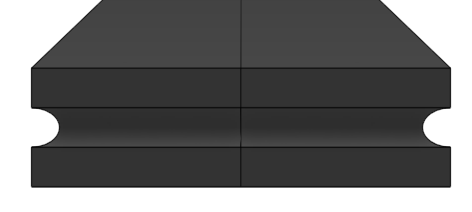
\includegraphics{../cut_images/base.png}
                    \caption{Base Image}
                \end{subfigure}
                \begin{subfigure}{.3\textwidth}
                    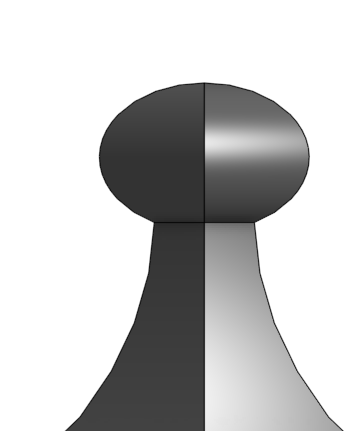
\includegraphics{../cut_images/pawn.png}
                    \caption{Pawn Image}
                \end{subfigure}
                \begin{subfigure}{.3\textwidth}
                    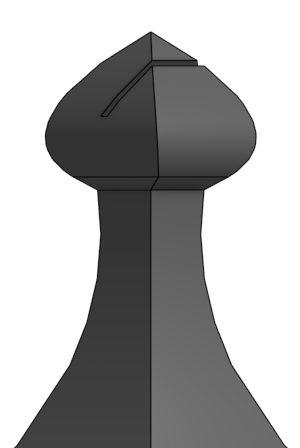
\includegraphics{../cut_images/bishop.png}
                    \caption{Bishop Image}
                \end{subfigure}
                \begin{subfigure}{.3\textwidth}
                    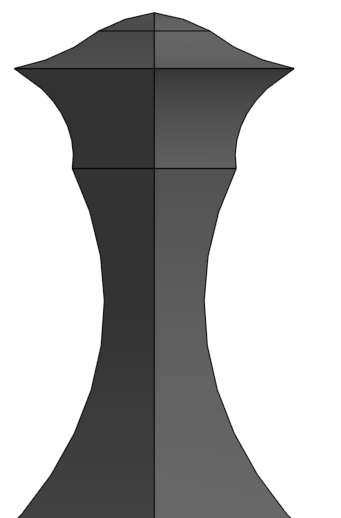
\includegraphics{../cut_images/queen.png}
                    \caption{Queen Image}
                \end{subfigure}
            \end{figure}
        
        \subsection{Measuring the Images}
            Each image was measured using Python 3 \footnote{https://www.python.org/} and OpenCV{https://opencv.org/}.  The image is measured in one-pixel tall layers, from the bottom
            of the image to the top.  For each layer, you can imagine a pair of calipers being used to measure the image; first the left jaw is brought in until it reaches a
            solid object(non-white pixel), then the process is repeated for the right jaw.  If both jaws touch the object, the distance between them is added to a list. If the jaws
            touch each other, the layer is empty, and ignored.  The measurements for each layer are returned in a list, in pixels, from bottom to top.  The code for this can be found in `code/measure.py'.
            
        \subsection{Scaling the Measurements}
            To reconstitute our measurements into g-code, each measurement must be scaled from a cross-section diagonal length in pixels, to a square side length, in millimeters.
            The formula for this is the following:
            $$ length_{side,mm} = \frac{\sqrt{2}}{2} \times length_{diagonal,px} \times \frac{millimeters}{pixel} $$
            The scaling factor, millimeters per pixel, was obtained using GIMP and `image\_info.txt'.  It is the given height of each piece divided by its height in pixels.  It appears
            that each piece has a different z scaling factor, but their x-y scaling factors are all the same.  The reason for this is not known, probably something to do with the render
            and export.  This was dealt with by running each model with its own z-scale.  This leads to a very small amount of error which we considered negligible.
            This scaling factor equation is applied to each measurement.  The python code for can be found in `code/scale.py'.

        \subsection{Building the Models}
            The models are built automatically layer by layer into OpenSCAD \footnote{https://www.openscad.org/} scripts.  Each measurement is constructed into a square prism with
            side lengths of each layer measurement, and a height equal to the scaled height of one pixel.  These prisms are stacked onto each other to form a model.  The OpenSCAD models are
            located in the `scad\_files' folder.  This python script is located in `code/export.py'  Each scad model is then manually exported as an STL to the `stls' folder.
            \begin{figure}
                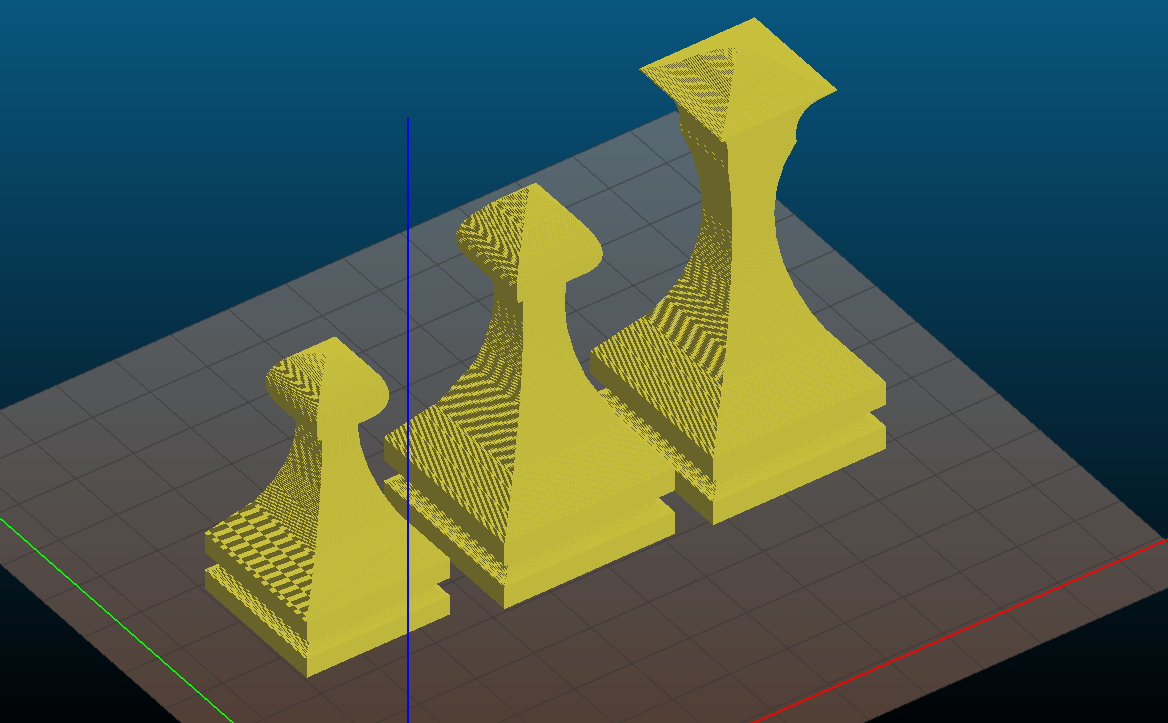
\includegraphics{../stls/stls.png}
                \caption{Models produced from Code}
            \end{figure}

        \subsection{Slicing and Solving}
            From the `damaged\_chess.gcode' file, we knew that the original g-code was sliced using slic3r, and the given settings were still intact.  Slic3r contains a settings
            recovery option, which was able to recover the settings.  The recovered settings are located in `settings/damaged\_chess.ini'.  Each model is manually sliced with the recovered
            settings.  The g-code for each model is stored in the `gcode' folder.  Slic3r calculates the amount of filament used, which is compared with the amount recovered from
            the damaged g-code to determine that the damaged g-code was from the queen.  The rebuilt g-code uses 4229.7mm of filament compared to the original model's 4290.7mm.  Using the formula
            $$ \%Error = 100 \times \frac{|length_{original} - length_{reconstructed|}}{length{reconstructed}} $$
            we achieve an error of just over 1\%.
            \begin{figure}
                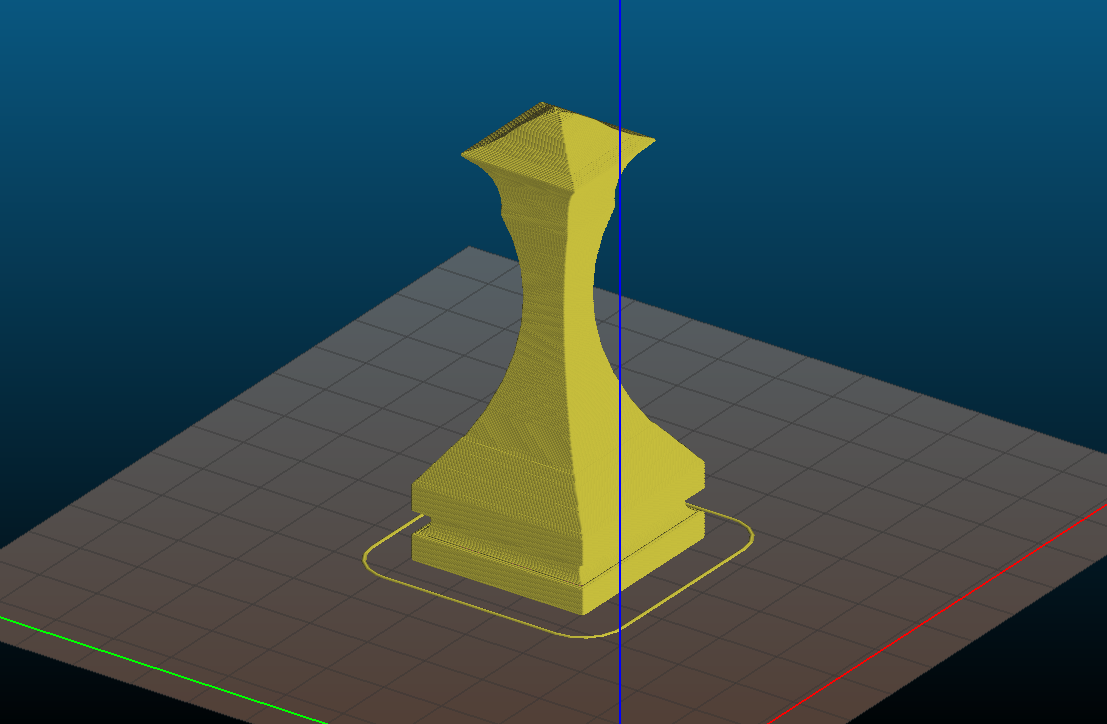
\includegraphics{../gcode/queen.png}
                \caption{G-code of Final Queen Model}
            \end{figure}

\end{document}